\documentclass[twoside]{book}

% Packages required by doxygen
\usepackage{fixltx2e}
\usepackage{calc}
\usepackage{doxygen}
\usepackage[export]{adjustbox} % also loads graphicx
\usepackage{graphicx}
\usepackage[utf8]{inputenc}
\usepackage{makeidx}
\usepackage{multicol}
\usepackage{multirow}
\PassOptionsToPackage{warn}{textcomp}
\usepackage{textcomp}
\usepackage[nointegrals]{wasysym}
\usepackage[table]{xcolor}

% Font selection
\usepackage[T1]{fontenc}
\usepackage[scaled=.90]{helvet}
\usepackage{courier}
\usepackage{amssymb}
\usepackage{sectsty}
\renewcommand{\familydefault}{\sfdefault}
\allsectionsfont{%
  \fontseries{bc}\selectfont%
  \color{darkgray}%
}
\renewcommand{\DoxyLabelFont}{%
  \fontseries{bc}\selectfont%
  \color{darkgray}%
}
\newcommand{\+}{\discretionary{\mbox{\scriptsize$\hookleftarrow$}}{}{}}

% Page & text layout
\usepackage{geometry}
\geometry{%
  a4paper,%
  top=2.5cm,%
  bottom=2.5cm,%
  left=2.5cm,%
  right=2.5cm%
}
\tolerance=750
\hfuzz=15pt
\hbadness=750
\setlength{\emergencystretch}{15pt}
\setlength{\parindent}{0cm}
\setlength{\parskip}{3ex plus 2ex minus 2ex}
\makeatletter
\renewcommand{\paragraph}{%
  \@startsection{paragraph}{4}{0ex}{-1.0ex}{1.0ex}{%
    \normalfont\normalsize\bfseries\SS@parafont%
  }%
}
\renewcommand{\subparagraph}{%
  \@startsection{subparagraph}{5}{0ex}{-1.0ex}{1.0ex}{%
    \normalfont\normalsize\bfseries\SS@subparafont%
  }%
}
\makeatother

% Headers & footers
\usepackage{fancyhdr}
\pagestyle{fancyplain}
\fancyhead[LE]{\fancyplain{}{\bfseries\thepage}}
\fancyhead[CE]{\fancyplain{}{}}
\fancyhead[RE]{\fancyplain{}{\bfseries\leftmark}}
\fancyhead[LO]{\fancyplain{}{\bfseries\rightmark}}
\fancyhead[CO]{\fancyplain{}{}}
\fancyhead[RO]{\fancyplain{}{\bfseries\thepage}}
\fancyfoot[LE]{\fancyplain{}{}}
\fancyfoot[CE]{\fancyplain{}{}}
\fancyfoot[RE]{\fancyplain{}{\bfseries\scriptsize Generated by Doxygen }}
\fancyfoot[LO]{\fancyplain{}{\bfseries\scriptsize Generated by Doxygen }}
\fancyfoot[CO]{\fancyplain{}{}}
\fancyfoot[RO]{\fancyplain{}{}}
\renewcommand{\footrulewidth}{0.4pt}
\renewcommand{\chaptermark}[1]{%
  \markboth{#1}{}%
}
\renewcommand{\sectionmark}[1]{%
  \markright{\thesection\ #1}%
}

% Indices & bibliography
\usepackage{natbib}
\usepackage[titles]{tocloft}
\setcounter{tocdepth}{3}
\setcounter{secnumdepth}{5}
\makeindex

% Hyperlinks (required, but should be loaded last)
\usepackage{ifpdf}
\ifpdf
  \usepackage[pdftex,pagebackref=true]{hyperref}
\else
  \usepackage[ps2pdf,pagebackref=true]{hyperref}
\fi
\hypersetup{%
  colorlinks=true,%
  linkcolor=blue,%
  citecolor=blue,%
  unicode%
}

% Custom commands
\newcommand{\clearemptydoublepage}{%
  \newpage{\pagestyle{empty}\cleardoublepage}%
}

\usepackage{caption}
\captionsetup{labelsep=space,justification=centering,font={bf},singlelinecheck=off,skip=4pt,position=top}

%===== C O N T E N T S =====

\begin{document}

% Titlepage & ToC
\hypersetup{pageanchor=false,
             bookmarksnumbered=true,
             pdfencoding=unicode
            }
\pagenumbering{alph}
\begin{titlepage}
\vspace*{7cm}
\begin{center}%
{\Large A\+CS B\+L\+DC Doxygen test }\\
\vspace*{1cm}
{\large Generated by Doxygen 1.8.13}\\
\end{center}
\end{titlepage}
\clearemptydoublepage
\pagenumbering{roman}
\tableofcontents
\clearemptydoublepage
\pagenumbering{arabic}
\hypersetup{pageanchor=true}

%--- Begin generated contents ---
\chapter{app\+\_\+template}
\label{index}\hypertarget{index}{}This is the template app for new applications.

To create a new app, simply copy the app\+\_\+template directory and name it whatever you like.


\begin{DoxyCode}
cp -R app\_template app\_<name>
\end{DoxyCode}


If building for a specific board, update the {\ttfamily B\+O\+A\+RD =} line to the board defined in the {\ttfamily boards} directory

Then, open the Makefile and edit the line {\ttfamily P\+R\+O\+J\+E\+CT =} to whatever name you chose\+: 
\begin{DoxyCode}
PROJECT   = app\_<name>
\end{DoxyCode}
 
\chapter{File Index}
\section{File List}
Here is a list of all files with brief descriptions\+:\begin{DoxyCompactList}
\item\contentsline{section}{\hyperlink{main_8c}{main.\+c} \\*B\+L\+DC control code }{\pageref{main_8c}}{}
\item\contentsline{section}{\hyperlink{structcmd_8h}{structcmd.\+h} \\*A Documented file }{\pageref{structcmd_8h}}{}
\end{DoxyCompactList}

\chapter{File Documentation}
\hypertarget{main_8c}{}\section{main.\+c File Reference}
\label{main_8c}\index{main.\+c@{main.\+c}}


B\+L\+DC control code.  


{\ttfamily \#include \char`\"{}ch.\+h\char`\"{}}\newline
{\ttfamily \#include \char`\"{}hal.\+h\char`\"{}}\newline
{\ttfamily \#include \char`\"{}chprintf.\+h\char`\"{}}\newline
{\ttfamily \#include \char`\"{}acs\+\_\+bldc.\+h\char`\"{}}\newline
Include dependency graph for main.\+c\+:\nopagebreak
\begin{figure}[H]
\begin{center}
\leavevmode
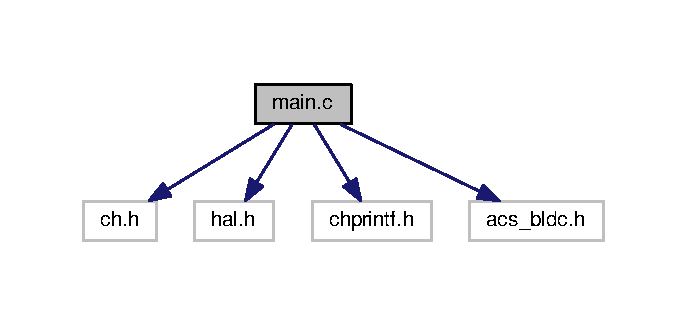
\includegraphics[width=330pt]{main_8c__incl}
\end{center}
\end{figure}
\subsection*{Functions}
\begin{DoxyCompactItemize}
\item 
static \hyperlink{main_8c_a0a81efa818549039218f68caf657552d}{T\+H\+D\+\_\+\+W\+O\+R\+K\+I\+N\+G\+\_\+\+A\+R\+EA} (wa\+\_\+bldc\+Thread, 128)
\item 
static \hyperlink{main_8c_a1989c402b1c29ba51d9a872513853457}{T\+H\+D\+\_\+\+F\+U\+N\+C\+T\+I\+ON} (bldc\+Thread, arg)
\item 
static void \hyperlink{main_8c_ad6cae3f4505c3e369a1ac0d3c3b60f42}{app\+\_\+init} (void)
\item 
static void \hyperlink{main_8c_a2e20249f9eb3339c1751ca1232ade7bc}{app\+\_\+main} (void)
\item 
int \hyperlink{main_8c_a840291bc02cba5474a4cb46a9b9566fe}{main} (void)
\end{DoxyCompactItemize}
\subsection*{Variables}
\begin{DoxyCompactItemize}
\item 
static Serial\+Config \hyperlink{main_8c_aac7dfdc32e0240ce7662d5a64f643608}{ser\+\_\+cfg}
\end{DoxyCompactItemize}


\subsection{Detailed Description}
B\+L\+DC control code. 

This file contains code that controls the B\+L\+D\+Cs (brushless DC motors). 

\subsection{Function Documentation}
\mbox{\Hypertarget{main_8c_ad6cae3f4505c3e369a1ac0d3c3b60f42}\label{main_8c_ad6cae3f4505c3e369a1ac0d3c3b60f42}} 
\index{main.\+c@{main.\+c}!app\+\_\+init@{app\+\_\+init}}
\index{app\+\_\+init@{app\+\_\+init}!main.\+c@{main.\+c}}
\subsubsection{\texorpdfstring{app\+\_\+init()}{app\_init()}}
{\footnotesize\ttfamily static void app\+\_\+init (\begin{DoxyParamCaption}\item[{void}]{ }\end{DoxyParamCaption})\hspace{0.3cm}{\ttfamily [static]}}


\begin{DoxyCode}
56                           \{
57     \textcolor{comment}{// Start up debug output}
58     bldcInit();
59     sdStart(&SD2, &\hyperlink{main_8c_aac7dfdc32e0240ce7662d5a64f643608}{ser\_cfg});
60 \}
\end{DoxyCode}
\mbox{\Hypertarget{main_8c_a2e20249f9eb3339c1751ca1232ade7bc}\label{main_8c_a2e20249f9eb3339c1751ca1232ade7bc}} 
\index{main.\+c@{main.\+c}!app\+\_\+main@{app\+\_\+main}}
\index{app\+\_\+main@{app\+\_\+main}!main.\+c@{main.\+c}}
\subsubsection{\texorpdfstring{app\+\_\+main()}{app\_main()}}
{\footnotesize\ttfamily static void app\+\_\+main (\begin{DoxyParamCaption}\item[{void}]{ }\end{DoxyParamCaption})\hspace{0.3cm}{\ttfamily [static]}}

Brief description. Brief description continued.

Detailed description starts here.

Begin main loop
\begin{DoxyCode}
62                           \{
70     chThdCreateStatic(
71         wa\_bldcThread,
72         \textcolor{keyword}{sizeof}(wa\_bldcThread), 
73         NORMALPRIO, 
74         bldcThread, 
75         NULL
76     );
77 
81     \textcolor{keywordflow}{while} (\textcolor{keyword}{true})\{
82         chThdSleepMilliseconds(1000);
83     \}
84 \}
\end{DoxyCode}
\mbox{\Hypertarget{main_8c_a840291bc02cba5474a4cb46a9b9566fe}\label{main_8c_a840291bc02cba5474a4cb46a9b9566fe}} 
\index{main.\+c@{main.\+c}!main@{main}}
\index{main@{main}!main.\+c@{main.\+c}}
\subsubsection{\texorpdfstring{main()}{main()}}
{\footnotesize\ttfamily int main (\begin{DoxyParamCaption}\item[{void}]{ }\end{DoxyParamCaption})}

System initializations.
\begin{DoxyItemize}
\item H\+AL initialization, this also initializes the configured device drivers and performs the board-\/specific initializations.
\item Kernel initialization, the \hyperlink{main_8c_a840291bc02cba5474a4cb46a9b9566fe}{main()} function becomes a thread and the R\+T\+OS is active.
\end{DoxyItemize}
\begin{DoxyCode}
86                \{
94     halInit();
95     chSysInit();
96     \textcolor{comment}{//oresat\_init(0);}
97 
98     \textcolor{comment}{//}
99     \textcolor{comment}{// Initialize and start app}
100     \hyperlink{main_8c_ad6cae3f4505c3e369a1ac0d3c3b60f42}{app\_init}();
101     \hyperlink{main_8c_a2e20249f9eb3339c1751ca1232ade7bc}{app\_main}();
102 
103     \textcolor{keywordflow}{return} 0;
104 \}
\end{DoxyCode}
\mbox{\Hypertarget{main_8c_a1989c402b1c29ba51d9a872513853457}\label{main_8c_a1989c402b1c29ba51d9a872513853457}} 
\index{main.\+c@{main.\+c}!T\+H\+D\+\_\+\+F\+U\+N\+C\+T\+I\+ON@{T\+H\+D\+\_\+\+F\+U\+N\+C\+T\+I\+ON}}
\index{T\+H\+D\+\_\+\+F\+U\+N\+C\+T\+I\+ON@{T\+H\+D\+\_\+\+F\+U\+N\+C\+T\+I\+ON}!main.\+c@{main.\+c}}
\subsubsection{\texorpdfstring{T\+H\+D\+\_\+\+F\+U\+N\+C\+T\+I\+O\+N()}{THD\_FUNCTION()}}
{\footnotesize\ttfamily static T\+H\+D\+\_\+\+F\+U\+N\+C\+T\+I\+ON (\begin{DoxyParamCaption}\item[{bldc\+Thread}]{,  }\item[{arg}]{ }\end{DoxyParamCaption})\hspace{0.3cm}{\ttfamily [static]}}


\begin{DoxyCode}
46                                    \{
47   (void)arg;
48   chRegSetThreadName(\textcolor{stringliteral}{"bldc"});
49 \textcolor{comment}{//  bldcSinStart();}
50     
51   \textcolor{keywordflow}{while}(!chThdShouldTerminateX())\{
52     chThdSleepMilliseconds(500);
53   \}
54 \}
\end{DoxyCode}
\mbox{\Hypertarget{main_8c_a0a81efa818549039218f68caf657552d}\label{main_8c_a0a81efa818549039218f68caf657552d}} 
\index{main.\+c@{main.\+c}!T\+H\+D\+\_\+\+W\+O\+R\+K\+I\+N\+G\+\_\+\+A\+R\+EA@{T\+H\+D\+\_\+\+W\+O\+R\+K\+I\+N\+G\+\_\+\+A\+R\+EA}}
\index{T\+H\+D\+\_\+\+W\+O\+R\+K\+I\+N\+G\+\_\+\+A\+R\+EA@{T\+H\+D\+\_\+\+W\+O\+R\+K\+I\+N\+G\+\_\+\+A\+R\+EA}!main.\+c@{main.\+c}}
\subsubsection{\texorpdfstring{T\+H\+D\+\_\+\+W\+O\+R\+K\+I\+N\+G\+\_\+\+A\+R\+E\+A()}{THD\_WORKING\_AREA()}}
{\footnotesize\ttfamily static T\+H\+D\+\_\+\+W\+O\+R\+K\+I\+N\+G\+\_\+\+A\+R\+EA (\begin{DoxyParamCaption}\item[{wa\+\_\+bldc\+Thread}]{,  }\item[{128}]{ }\end{DoxyParamCaption})\hspace{0.3cm}{\ttfamily [static]}}



\subsection{Variable Documentation}
\mbox{\Hypertarget{main_8c_aac7dfdc32e0240ce7662d5a64f643608}\label{main_8c_aac7dfdc32e0240ce7662d5a64f643608}} 
\index{main.\+c@{main.\+c}!ser\+\_\+cfg@{ser\+\_\+cfg}}
\index{ser\+\_\+cfg@{ser\+\_\+cfg}!main.\+c@{main.\+c}}
\subsubsection{\texorpdfstring{ser\+\_\+cfg}{ser\_cfg}}
{\footnotesize\ttfamily Serial\+Config ser\+\_\+cfg\hspace{0.3cm}{\ttfamily [static]}}

{\bfseries Initial value\+:}
\begin{DoxyCode}
= \{
    115200,     
    0,          
    0,          
    0,          
\}
\end{DoxyCode}

\hypertarget{README_8md}{}\section{R\+E\+A\+D\+M\+E.\+md File Reference}
\label{README_8md}\index{R\+E\+A\+D\+M\+E.\+md@{R\+E\+A\+D\+M\+E.\+md}}

\hypertarget{structcmd_8h}{}\section{structcmd.\+h File Reference}
\label{structcmd_8h}\index{structcmd.\+h@{structcmd.\+h}}


A Documented file.  


\subsection*{Macros}
\begin{DoxyCompactItemize}
\item 
\#define \hyperlink{structcmd_8h_afa99ec4acc4ecb2dc3c2d05da15d0e3f}{M\+AX}(a,  b)~(((a)$>$(b))?(a)\+:(b))
\begin{DoxyCompactList}\small\item\em A macro that returns the maximum of {\itshape a} and {\itshape b}. \end{DoxyCompactList}\end{DoxyCompactItemize}
\subsection*{Typedefs}
\begin{DoxyCompactItemize}
\item 
typedef unsigned int \hyperlink{structcmd_8h_ae1e6edbbc26d6fbc71a90190d0266018}{U\+I\+N\+T32}
\begin{DoxyCompactList}\small\item\em A type definition for a . \end{DoxyCompactList}\end{DoxyCompactItemize}
\subsection*{Functions}
\begin{DoxyCompactItemize}
\item 
int \hyperlink{structcmd_8h_a2c4414339f388561554c2deab11a1a07}{open} (const char $\ast$, int)
\begin{DoxyCompactList}\small\item\em Opens a file descriptor. \end{DoxyCompactList}\item 
int \hyperlink{structcmd_8h_ae152484c890a24e4d9b4980e7b965be0}{close} (int)
\begin{DoxyCompactList}\small\item\em Closes the file descriptor {\itshape fd}. \end{DoxyCompactList}\item 
size\+\_\+t \hyperlink{structcmd_8h_af2a3ea719b83f672637febdd87c36c36}{write} (int, const char $\ast$, size\+\_\+t)
\begin{DoxyCompactList}\small\item\em Writes {\itshape count} bytes from {\itshape buf} to the filedescriptor {\itshape fd}. \end{DoxyCompactList}\item 
int \hyperlink{structcmd_8h_a9c7b76d5266903891c803132d51ccb90}{read} (int, char $\ast$, size\+\_\+t)
\begin{DoxyCompactList}\small\item\em Read bytes from a file descriptor. \end{DoxyCompactList}\end{DoxyCompactItemize}
\subsection*{Variables}
\begin{DoxyCompactItemize}
\item 
int \hyperlink{structcmd_8h_ad65a8842cc674e3ddf69355898c0ecbf}{errno}
\begin{DoxyCompactList}\small\item\em Contains the last error code. \end{DoxyCompactList}\end{DoxyCompactItemize}


\subsection{Detailed Description}
A Documented file. 

Details. 

\subsection{Macro Definition Documentation}
\mbox{\Hypertarget{structcmd_8h_afa99ec4acc4ecb2dc3c2d05da15d0e3f}\label{structcmd_8h_afa99ec4acc4ecb2dc3c2d05da15d0e3f}} 
\index{structcmd.\+h@{structcmd.\+h}!M\+AX@{M\+AX}}
\index{M\+AX@{M\+AX}!structcmd.\+h@{structcmd.\+h}}
\subsubsection{\texorpdfstring{M\+AX}{MAX}}
{\footnotesize\ttfamily \#define M\+AX(\begin{DoxyParamCaption}\item[{}]{a,  }\item[{}]{b }\end{DoxyParamCaption})~(((a)$>$(b))?(a)\+:(b))}



A macro that returns the maximum of {\itshape a} and {\itshape b}. 

Details. 

\subsection{Typedef Documentation}
\mbox{\Hypertarget{structcmd_8h_ae1e6edbbc26d6fbc71a90190d0266018}\label{structcmd_8h_ae1e6edbbc26d6fbc71a90190d0266018}} 
\index{structcmd.\+h@{structcmd.\+h}!U\+I\+N\+T32@{U\+I\+N\+T32}}
\index{U\+I\+N\+T32@{U\+I\+N\+T32}!structcmd.\+h@{structcmd.\+h}}
\subsubsection{\texorpdfstring{U\+I\+N\+T32}{UINT32}}
{\footnotesize\ttfamily typedef unsigned int \hyperlink{structcmd_8h_ae1e6edbbc26d6fbc71a90190d0266018}{U\+I\+N\+T32}}



A type definition for a . 

Details. 

\subsection{Function Documentation}
\mbox{\Hypertarget{structcmd_8h_ae152484c890a24e4d9b4980e7b965be0}\label{structcmd_8h_ae152484c890a24e4d9b4980e7b965be0}} 
\index{structcmd.\+h@{structcmd.\+h}!close@{close}}
\index{close@{close}!structcmd.\+h@{structcmd.\+h}}
\subsubsection{\texorpdfstring{close()}{close()}}
{\footnotesize\ttfamily int close (\begin{DoxyParamCaption}\item[{int}]{fd }\end{DoxyParamCaption})}



Closes the file descriptor {\itshape fd}. 


\begin{DoxyParams}{Parameters}
{\em fd} & The descriptor to close. \\
\hline
\end{DoxyParams}
\mbox{\Hypertarget{structcmd_8h_a2c4414339f388561554c2deab11a1a07}\label{structcmd_8h_a2c4414339f388561554c2deab11a1a07}} 
\index{structcmd.\+h@{structcmd.\+h}!open@{open}}
\index{open@{open}!structcmd.\+h@{structcmd.\+h}}
\subsubsection{\texorpdfstring{open()}{open()}}
{\footnotesize\ttfamily int open (\begin{DoxyParamCaption}\item[{const char $\ast$}]{pathname,  }\item[{int}]{flags }\end{DoxyParamCaption})}



Opens a file descriptor. 


\begin{DoxyParams}{Parameters}
{\em pathname} & The name of the descriptor. \\
\hline
{\em flags} & Opening flags. \\
\hline
\end{DoxyParams}
\mbox{\Hypertarget{structcmd_8h_a9c7b76d5266903891c803132d51ccb90}\label{structcmd_8h_a9c7b76d5266903891c803132d51ccb90}} 
\index{structcmd.\+h@{structcmd.\+h}!read@{read}}
\index{read@{read}!structcmd.\+h@{structcmd.\+h}}
\subsubsection{\texorpdfstring{read()}{read()}}
{\footnotesize\ttfamily int read (\begin{DoxyParamCaption}\item[{int}]{fd,  }\item[{char $\ast$}]{buf,  }\item[{size\+\_\+t}]{count }\end{DoxyParamCaption})}



Read bytes from a file descriptor. 


\begin{DoxyParams}{Parameters}
{\em fd} & The descriptor to read from. \\
\hline
{\em buf} & The buffer to read into. \\
\hline
{\em count} & The number of bytes to read. \\
\hline
\end{DoxyParams}
\mbox{\Hypertarget{structcmd_8h_af2a3ea719b83f672637febdd87c36c36}\label{structcmd_8h_af2a3ea719b83f672637febdd87c36c36}} 
\index{structcmd.\+h@{structcmd.\+h}!write@{write}}
\index{write@{write}!structcmd.\+h@{structcmd.\+h}}
\subsubsection{\texorpdfstring{write()}{write()}}
{\footnotesize\ttfamily size\+\_\+t write (\begin{DoxyParamCaption}\item[{int}]{fd,  }\item[{const char $\ast$}]{buf,  }\item[{size\+\_\+t}]{count }\end{DoxyParamCaption})}



Writes {\itshape count} bytes from {\itshape buf} to the filedescriptor {\itshape fd}. 


\begin{DoxyParams}{Parameters}
{\em fd} & The descriptor to write to. \\
\hline
{\em buf} & The data buffer to write. \\
\hline
{\em count} & The number of bytes to write. \\
\hline
\end{DoxyParams}


\subsection{Variable Documentation}
\mbox{\Hypertarget{structcmd_8h_ad65a8842cc674e3ddf69355898c0ecbf}\label{structcmd_8h_ad65a8842cc674e3ddf69355898c0ecbf}} 
\index{structcmd.\+h@{structcmd.\+h}!errno@{errno}}
\index{errno@{errno}!structcmd.\+h@{structcmd.\+h}}
\subsubsection{\texorpdfstring{errno}{errno}}
{\footnotesize\ttfamily int errno}



Contains the last error code. 

\begin{DoxyWarning}{Warning}
Not thread safe! 
\end{DoxyWarning}

%--- End generated contents ---

% Index
\backmatter
\newpage
\phantomsection
\clearemptydoublepage
\addcontentsline{toc}{chapter}{Index}
\printindex

\end{document}
